\chapter{功利主義}




\section{ベンサム『道徳と立法の原理序説』 (1789)}

ジェレミー・ベンサム (Jeremy Bentha, 1748--1832)。

出典:ベンサム『道徳および立法の諸原理序説』、『中公世界の名著38 ベンサム・ミル』所収、山下一重訳、中央公論社、1967。

\subsection{}


    自然は人類を\kenten{苦痛}と\kenten{快楽}という、二人の主権者の支配のもとにおいてきた。われわれが何をしなければならないかということを指示し、またわれわれが何をするであろうかということを決定するのは、ただ苦痛と快楽だけである。一方においては善悪の基準が、他方においては原因と結果の連鎖が、この二つの玉座につながれている。苦痛と幸福とは、われわれのするすべてのこと、われわれの言うすべてのこと、われわれの考えるすべてのことについて、われわれを支配しているのであって、このような従属をはらいのけようとどんなに努力しても、その努力はこのような従属を証明し、確認するのに役だつだけであろう。ある人は、ことばのうえではこのような帝国を放棄したように見せかけるかもしれないが、実際上は依然としてその帝国に従属しつづけている。


     \begin{figure}[htbp]
       \centering
         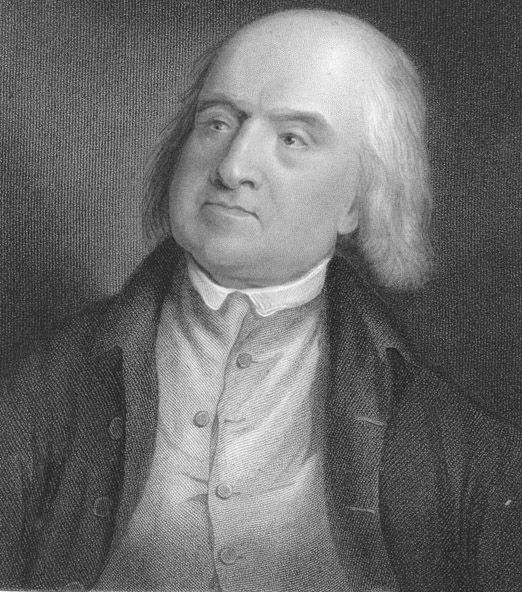
\includegraphics[width=50mm]{images/bentham.jpg}
       \caption{ベンサム}
     \end{figure}

\subsection{}

\emph{二} 功利性の原理とは、その利益が問題になっている人々の幸福を、増大させるように見えるか、それとも減少させるように見えるかの傾向によって、または同じことを別のことばで言いかえただけであるが、その幸福を促進するようにみえるか、それともその幸福に対立するようにみえるかによって、すべての行為を是認し、または否認する原理を意味する。私はすべての行為と言った。したがって、それは、一個人のすべての行為だけでなく、政府のすべての政策をも含むのである。……

\emph{四} 社会の利益とは、道徳に関する用語法に出てくる、もっとも一般的な表現の一つである。このことばの意味が見失われて、はっきりしなくなることがよくあるが、それも不思議なことではない。社会の利益ということばが意味をもつのは、次のような場合である。社会とは、いわばその\kenten{成員}を構成すると考えられる個々の人々から構成される、擬制的な\kenten{団体}である。それでは、社会の利益とはなんであろうか。それは社会を構成している成員の利益の総計にほかならない。(83)





\subsection{}

政府の仕事は、刑罰と報償によって、社会の幸福を促進することである。政府の仕事のうち、刑罰に関する部分は、特に刑法の対象である。ある行為が社会の幸福を阻害する傾向が大きければ大きいほど、その傾向が有害であればあるほど、その行為が呼び起こす刑罰の必要は大きいであろう。(148)





\newpage{}
\section{J. S. ミル『自由論』 (1859)}


J. S. ミル (John Stuart Mill, 1806--1873)。

出典:J. S. ミル『自由論』、『中公世界の名著38 ベンサム・ミル』所収、早坂忠訳、中央公論社、1967。






     \begin{figure}[htbp]
       \centering
         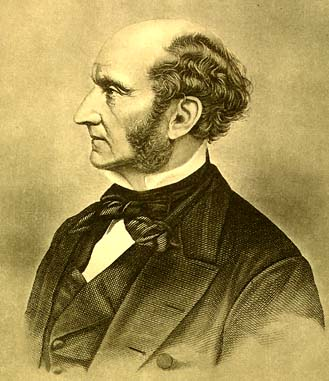
\includegraphics[width=50mm]{images/JohnStuartMill.jpg}
       \caption{J. S. ミル}
     \end{figure}


\subsection{危害原理}



この論文の目的は、用いられる手段が、法的刑罰という形の物理的力であれ、世論という道徳的強制であれ、強制と統制という形での個人に対する社会の取扱いを絶対的に支配する資格のある、一つの非常に単純な原理を主張することである。その原理とは、人類が、個人的にまたは集団的に、だれかの行動の自由に正当に干渉しうる唯一の目的は、自己防衛だということである。すなわち、文明社会の成員に対し、彼の意志に反して、正当に権力を行使しうる唯一の目的は、他人にたいする危害の防止である。彼自身の幸福は、物質的なものであれ道徳的なものであれ、十分な正当化となるものではない。そうするほうが彼のためによいだろうとか、彼をもっとしあわせにするだろうとか、他の人々の意見によれば、そうすることが賢明であり正しくさえあるからといって、彼になんらかの行動や抑制を強制することは、正当ではありえない。(『自由論』第1章)


\subsection{言論・表現の自由の必要性}


新教徒なら少なくとも否定しないことだが、もし人類の知性と判断力が育成さるべきだとすれば、だれの場合でも、自分に大いに関係があり自分の意見をもたねばならぬ、と考えられている事がらにおいてこそ、これらの能力がもっとも適切に訓練されるのではないだろうか。理解力の育成が、他の何ものよりも、ある一つのものにかかっているとすれば、たしかにそれは、自己の意見の根拠を知ることにかかっているのである。人びとは、何を信じようとも、正しく信じることが第一に重要である問題に関しては、少なくともふつうの反対意見に対しては、自己を擁護することができなくてはならない。

しかし、次のように言う人があるかもしれない。人びとは、彼らの意見の根拠を\kenten{教え}られればよいではないか。意見が反駁されるのをきいたことがないからといって、それらの意見が、ただわけもなく繰り返されるにちがいないということにはならない。幾何学を学ぶ人びとは、単に定理を暗記するだけでなく、証明をも同様に理解し覚えるのである。だから、幾何学の真理がだれかによって否定されたり反証を試みられたりしたのを彼らがきいたことがないからといって、彼らがその真理の根拠を知らずにいるのだというのは、ばかげているだろう」と。たしかにそのとおりである。そして数学のような問題については、このような教え方で十分なのである。そこでは、まちがっている側には、いっさい弁明の余地がないのだ。数学的真理の証明の特異性は、そこには一方的議論しかない、ということである。反論もなければ、反論に対する回答もないのである。


しかし、意見の相違が可能なあらゆる問題については、真理は、相争う二組の理由のあいだに見いだされる差額の大きさに依存している。物理学においてさえ、同一の事実について、何か他の説明がつねに可能である。太陽中心説のかわりに地球中心説、酸素のかわりにフロジストン、というように。したがって、その他方の理論がなぜ正しい理論ではありえないのか、が明らかにされねばならない。このことが明らかにされるまでは、そしてどのように明らかにされるかを知るまでは、われわれは、われわれの意見の根拠を理解してはいないのである。だが、もっと無限に複雑な問題、すなわち道徳、宗教、政治、社会関係、生活上の問題になると、問題とされている意見を支持する議論の四分の三までは、それと異なるなんらかの意見に有利な状況を排除することからなっている。古代で一人(デモステネス)に次ぐ最大の雄弁家(キケロ)は、彼の論敵の主張を、自分のそれよりいっそう熱心とはいわぬまでも、同様の熱心さで研究した、と記録にのこしている。キケロが弁論の成功の手段として実行したことは、真理に到達することを目的としてなんらかの問題を研究するすべての人によって、見習われなければならない。

問題の自分自身の側しか知らない人は、それについてはほとんど何も知ってはいないのである。彼の理由は正しいものであり、また、だれもそれを反駁することができなかったかもしれない。しかし、もし彼が、反対側の理由を論駁することが、同じようにできないとすれば、そして反対側の理由が何なのかさえ知らないとれば、彼には、どちらか一方の意見を選ぶ理由もないのである。彼は権威に導かれるか、世間一般と同じように、自分がもっともひきつけられると感ずる側をとるか、のいずれかである。

\vspace{1zw}

……一般に受け入れられている意見が正しいときに、自由な討論のないことがひき起こす有害な作用が、もし、人びとがそれらの意見の根拠を知らされずにいるということに限られているとすれば、次のような考え方が生まれるかもしれない。これは、知的な悪ではあってもけっして道徳的な悪ではなく、人間への影響という点からみれば、それらの意見の価値を左右するものではないのだ、と。しかし実際は、討論が行なわれない場合には、意見の根拠が忘れられるだけではなく、意見の意味それ自体があまりにもしばしば忘れらてしまうのである。その意見を伝えることばは、なんの思想をも示唆しなくなってしまうか、あるいは本来それを伝えるためにそれらのことばが用いられていた思想の、ごく一部分しか示唆しなくなる。鮮明な概念と生きた信念のかわりに、機械的暗記で記憶された二、三の語句が残るだけになる。あるいは、たとえいくらか残ったとしても、意味のぬけがらと皮だけが残り、もっとすぐれた本質は失われる。……

\section*{幸福の一要素としての個性について}

……以上が、人類が自由に意見を形成し、その意見をはばかることなく発表することを絶対必要とする理由である。また以上が、この自由が承認されるかあるいは禁止をもかえりみず主張されるのでないかぎり、人間の知的本性に対して、またそれを通じて道徳的本性に対してもたらされる有害な影響である。そこで、われわれは次に、同じ理由が、人間が自己の意見にもとづいて自由に行動するべきことを、つまり自己の危険と責任とにおいてなされるかぎり、同胞から肉体的にであれ精神的にであれ妨害されることなしに、自己の意見を生活の中で自由に実行に移すべきことを、要求するのではなかろうか、ということを検討してみよう。



自己の危険と責任とにおいて、というこの条件は、いうまでもなく、絶対に必要である。誰も、行為が意見と同じように自由であるべきだ、と主張しはしない。反対に、意見でさえ、その発表が何か有害な行為を積極的に誘発するような事情があるときには、他から干渉されずにすむという権利を失うのである。穀物商人は、貧民を飢えさせる者であるとか、私有財産は略奪であるという意見は、単に出版物を通じて流布されるだけなら妨害されるべきではないが、穀物商人の家の前に集まった興奮した群集に対して口から伝えられたり、その中でプラカードという形で伝えられたりする場合には、当然罰を受けてよい。正当な理由なしに他人に害を与えるような行為は、どんな種類のものであれ、これに反対する感情によって、また必要ならば人々の積極的干渉によって抑制されてよいし、またより重要ないくつかの場合には抑制されることが絶対に必要である、個人の自由はここまでは制限されなければならない。彼は自己を他人にとっての邪魔ものにしてはならないのである。


しかし、もし個人が、他人に関係する事がらで他人を邪魔することを慎み、ただ自分自身にのみ関係する事がらで自己の性向と判断とにしたがって行動するだけだとすれば、意見が自由でなければならぬことを示すと同一の理由が、彼は自己の責任で自分の意見を邪魔されることなしに実行に移すことを許されるべきだ、ということをも明らかにするのである。人類は無誤謬ではないこと、彼らの真理は大部分は半真理にすぎぬこと、意見の一致は相反する意見のもっとも十分でもっとも自由な比較対象から生じたものでないかぎり望ましいものではないこと、また真理のあらゆる側面を認識する人類の能力が今日よりずっと増すまでは多様性は悪ではなくて善であること、これらのことは、人間の意見に対してと同様、その行動の様式に対しても適用される原理である。


人類が、不完全であるかぎりは、さまざまな意見のあることが有益であるのと同じく、次のことが有益である。すなわち、さまざまな生活の実験があること、他人への危害がないかぎり自由な活動の場が多種多様な性格に対して与えられること。また、さまざまな生活様式をもし試みるのが適当と思う人があれば実際にやってみてその価値を明らかにすること、が有益である。要するに、第一義的に他人に関係しない事柄においては、個性が自己を主張することが、望ましい。その人自身の性格ではなくてほかの人々の伝統や慣習が行為の規則となっているところでは、人間の幸福の主要な構成要素の一つであり、かつ個人的社会的進歩のまさに第一の構成要素をなすものが、欠けていることになるのである。


この原理を主張する際に出会う最大の困難は、ある承認された目的に達するための手段の正しい理解にあるのではなく、目的そのものに対する一般の人々の無関心にある。もし個性の自由な発展が幸福のもっとも本質的な要素の一つであると感じられているとすれば、またもしそれが文明、指導、教育、教養などのことばによってあらわされるすべてものもと同等の一要素であるのみならず、それ自体これらのものすべての必要な部分であり条件であると感じられているとすれば、自由が過小評価されるおそれはないだろうし、自由と社会的統制との境界を調整することが異常な困難を生むこともないであろう。


しかし困ったことには、ふつうの考え方によっては、個人の自発性がなんらかの本質的な価値をもつものであるとか、それ自体尊重に値するものである、とはほとんど認められていないのである。大多数の人々は、現在あるがままの人類の行き方に満足しているので〔というのは彼らこそがそれを現在あるがままのものにしている人々なのであるから〕、なぜこの生き方があらゆる人々にとって十分よいものでないのかを理解することができない。そのうえ、自発性は、道徳的社会的改革家の大多数をなす人々の理想の一部とはなっていない。むしろそれは、これらの改革家たちが人類にとって最善のものだと独断的に考えるものを一般に受け入れさせる場合の、厄介なそしておそらくそれにさからう障害として警戒心をもって見られているのである。


ドイツ以外ではほとんどの人が、\ruby{碩学}{せきがく}としても政治家としてもほまれの高いヴィルヘルム・フォン・フンボルト\footnote{一七六七〜一八三五。ドイツの人文主義者、政治家、言語学者。}が、ある論著の趣旨とした次のような学説の意味を、理解することさえできない。すなわち、「人間の目的、つまり理性の永遠普遍の命令によって規定されており、あいまいな一時的欲求によって示唆されたのではない目的は、人間の諸能力を、完全で矛盾のない全体へと最高度に、もっとも調和的に発展させることである」。したがって、「あらゆる人間がたえず努力を向けなければならず、また特に同胞に影響を与えようとする人々がつねに注意を払わなければならない」目標は、「能力と発展の個性である」。このためには、「自由および境遇の多様性」という二つの必要能力がある。そして、この二つの結合から、「個性の活力と豊かな多様性」が生まれ、これが結合して「独創性」となる、というのである。

しかしながら、人々がフォン・フンボルトのような学説にはほとんどなじみがないとしても、また個性にそのような高い価値をおくことが彼らにとっておどろくべきことであるとしても、それにかかわらずわれわれは、問題は単なる程度の問題なのだと考えなければならない。行為の卓越性についてのだれの考えをとってみても、人は互いに模倣しあう以外に絶対に何事もすべきではない、などと言う人はいない。だれも、人は自己の生活様式や自己の問題の処理の中に、自己自身の判断や自己自身の個性をいささかももちこむべきではない、などと主張しはしないであろう。他方、人が、自分が生まれる以前には、この世界では何一つわかっていなかったかのように、またある生活様式や行為の様式が他のそれよりもすぐれていることを示すために、経験がまだ何ごともしてこなかったかのように生活すべきだ、と主張するのも愚かしいであろう。人類の経験によってたしかめられた成果を知って利益を得るように、人は若いときに教えられ訓練されなければならぬ、ということはだれも否定はしない。


しかし、経験を自分自身の仕方で活用し解釈することは、諸能力が成熟に達した人間の特権であり正当な条件である。記録されている経験のどの部分が彼自身の境遇と性格に正しく適用されるかを見つけるのは、彼の仕事である。他の人々の伝統や習慣は、ある程度まで、彼らの経験が何を\kenten{彼らに}教えてきたかを示す証拠である。それは、推定証拠ではあるが、そのようなものとして、人の尊敬を要求する。しかし、第一に、彼らの経験はせますぎるかもしれぬし、また彼らはそれを正しく解釈してこなかったかもしれない。第二に、経験についての彼らの解釈は正しいかもしれぬが、彼には適当でないかもしれない。習慣は通例の環境と通例の性格とのためにつくられるものであるが、彼の環境や彼の性格は通例のものでないかもしれないのである。第三に、その習慣が習慣としてよいものであり、また彼に適合するとしても、ただ単に習慣\kenten{だからという理由で}それに同調することは、人間にのみ与えられた諸能力のどれをも彼の中に育成し発展させることにはならないのである。

知覚、判断、識別感情、精神活動、倫理的好悪さえも含めた人間の諸能力は、選択という行為をする際にのみ訓練される。何事であれそうするのが習慣だからといってする人は、なんの選択もしない。彼は最善のものを見わけたり望んだりする練習ができない。肉体的能力と同じように精神的道徳的能力も、使われることによってのみ向上する。ただ、他の人々がするからするというのでは、これらの能力は少しも訓練されない。それはちょうどある事がらを、他の人々がそれを信じているという理由だけで信じるのど同様である。もしある意見の根拠が、その人自身の理性を納得させるものでなえければ、彼の理性はその意見を採用することによって強められはせず、むしろ弱められがちである。そして、行為への誘因が彼自身の感情や性格に一致しないようなものならば、〔愛情や他人の権利が関係していない場合〕それは彼の感情や性格を活発で精力的なものにするかわりに、不活発で鈍いものにするのに大いに役だつのみである。

自己の生活設計を、自分のかわりに、世間や自分自身が属している世間の一部が選ぶのにまかせる人は、\ruby{猿}{さる}のような模倣能力のほかにはどんな能力も必要としない。自分自身で生活設計を選ぶ人は、彼のすべての能力を使用する。彼は、見る観察力、予測する推理力と判断力、決定に必要な資料を集める活動力、決定する識別力を使わなければならず、いったん決定をくだしたら、自己の熟慮した決定を守る確固とした意思と自制心を使わなければならない。そして、彼はこれらの能力を、自己の行為のうち、みずからの判断と感情にもとづいて決定する部分の大きさに比例して必要とし、また行使するのである。

これらの能力が何もなくとも、彼がある立派な道に導かれ邪道に陥らぬようにされるということはありうる。しかしそれでは、彼の人間としての他とは異なった価値はなんになるのであろうか。人が何をするかということのみならず、それをするのがどのような人々なのかということも真に重要なのである。人の生活が、その完成と美化とのために正当に用いられる人間の様々な製作品の中で、もっとも重要なものは、疑いもなく人間自身である。家を建て、穀物を栽培し、戦争を行い、訴訟を裁判し、さらに教会を建て祈祷をすることさえをも機械にさせることが{\——}人間の形をした自動人形にさせることが可能であると仮定しよう。そうであるとしても、今日、世界のより文明の開けた部分に住んでいる男女であって、たしかに自然が生むことができ、また、生むであろうものの貧弱な見本にすぎないような人々をすら、これらの自動人形でおきかえるのは、少なからぬ損失であろう。人間の本性は、ひな形にならって組み立てられ、自己に定められた仕事だけを正確にするように作られている機械ではない。それは一本の樹木であり、それ自身を生命あるものとしている内面の力の\ruby{趨勢}{すうせい}にしたがって、あらゆる側面にわたってみずから成長し発展することをもとめているものなのである。



人々が、彼らの理解力を行使することが望ましいということ、そしてまた、習慣に理性的にしたがうこと、ないしときには習慣から理性的に逸脱することすらもが、盲目的にただ機械的にそれをしたがうよりもよいということは、おそらく認められるであろう。われわれの理解力はわれわれ自身のものであるべきだ、ということはある程度までは認められている。しかし、われわれの願望や衝動もまた同様にわれわれ自身のものでなければならぬということ、あるいはわれわれ自身の、しかもなんらかの力を持った衝動を持つことは決して危険でも誘惑でもないということに対しては、それを認めようとする前と同様の積極的気持ちがみられない。


しかしながら、願望や衝動とて、信念や自制心とまったく同様に、完全な人間の一部分なのである。そして、強い衝動が危険なのは、それが正しいバランスを保っていないとき、つまり一組の目標と成功が発展して力強いものとなっているのに、それと共存すべき他の一組が弱く不活発なままであるときだけである。人々が誤った行動をとるのは、願望が強いからではない。良心が弱いからである。強い衝動と弱い良心とのあいだにはなんの自然的つながりもない。自然的つながりはその逆である。ある人の願望と感情が他の人のそれらより強く変化に富んでいる、ということは、その人のほうが人間性の素材をより多くもっており。したがってより多くの悪もなしうるかもしれぬが、確実により多くの善をもなすことができる、ということにほかならない。強い衝動とは精力の別名にすぎない。精力は誤った目的に用いられることもあろう。しかし、精力的な性格は、怠惰で無感覚な性格よりもつねに多くの善を産みだしうる。自然な感情をもっとも多くもつ人々は、つねに、その\ruby{陶冶}{とうや}された感情がもっとも強烈なものになされうる人々である。個人的衝動を生き生きと力あふれたものにすると同一の強い感受性が、また、徳へのもっとも熱烈な愛と、もっとも厳格な自制心とを生む源泉なのである。社会がその義務を果たしその利益を守るのは、これらのものを養成することによってなのであって、英雄をつくるすべが社会にわからないという理由から、英雄のつくられる素材を拒否することによってなのではない。


願望と衝動とが自分自身のものである人、自分自身の育成によって発展させられ、変化させられてきた彼自身の本性のあらわれが、彼自身の願望と衝動とになっている人は、性格をもつといわれる。願望と衝動が彼自身のものでない人は性格をもたない。それは、蒸気機関が性格をもたないのと同様である。もし、彼の衝動が彼自身のものであるというだけでなく、強烈なものであり、しかも強固な意志の支配下にあるならば、彼は精力的な性格をもつ。さまざまな、願望や衝動をもつ個性の開花は、奨励されるべきではないと考える人がいるとすれば、それらの人々はすべて次のことを主張しているのにほかならない。すなわち、社会は力強い本性なんら必要としてはいない{\——}のだし、また精力の一般的平均が高いことは望ましいことではないのだ、と。


% 初期の若干の社会状態においては、このような願望や衝動が、当時の社会の持っていた、それを訓練し統制する力をはるかにしのいでいたかもしれないし、また事実そのような場合もあった。自発性と個性の要素が過度にあって、社会的原理がそれとはげしくたたかった時代があった。そのときの困難な、力強い肉体と精神をもつ人々を動かして、その衝動の抑制を求めるなんらかの規則に彼らを服従させることであった。この困難に打ち勝つために法と規律は、皇帝たちと争う教皇たちのように、全人格を支配する権力を主張し、彼の性格をおさえるために彼の全生活を支配することを要求したのである{\——}これ以外にそれを統制しうる十分な手段を社会は見いだしていなかったのである。


% だが今日、社会はかなりの程度まで個性に対して勝利をおさめている。そして、人間性をおびやかしている危険は、個人的な衝動や好みが多すぎることではなく、それが不足していることである。地位や個人的\ruby{天賦}{てんぶ}によって強者だった人々の情熱がたえず法律や命令に反抗する立場にたち、彼らの情熱のおよぶ範囲内の人々がいくらかでも安定した生活を享受しうるためには、その情熱を厳格にくさりでつないでおく必要があった時代とくらべて、事態は大きく変化している。われわれの時代においては、社会の最高の階級から最低の階級に至るまで、だれもが、敵意にみちたおそろしい監視のもとに暮らしているかのようである。他人に関係することだけでなく彼ら自身だけに関係することであっても、個人も家族も次のようにみずからにたずねはしない{\——}私は何を好むのか、何が私の性格や気質に合うのだろうか、何が私のうちにある最善にして最高のものを十分に活動させそれが成長し栄えるのを可能にするのであろうか、と。彼らは、みずからに向かってこうたずねるのである。何が私の地位にふさわしいだろうか、私と同じような身分と経済状態にある人々は何をするのがふつうだろうか、あるいは〔さらに悪いことには〕私より上の身分と経済状態にある人々は何をするのがふつうだろうか、と。


% 私は、彼らが彼ら自身の成功に合うものを捨てて慣習的のものを選ぶ、といっているのではない。彼らは、慣習的なものに対するものをのぞけば、なんの性向をももとうとはしないのである。このように精神自身がくびきに屈しているのである。人々が楽しみのためにすることにおいてさえ、他との一致ということがまず第一に考えられる。彼ら群衆の好みにしたがって好む。彼らは、ふつう一般に行われることの中からしか選択しない。特異な趣味や\ruby{奇矯}{ききょう}な行為は、犯罪と同様に忌避される。ついには、自己の本性にしたがわぬことによって、彼らはしたがうべき本性をもたなくなる。彼らの人間的諸能力はしぼみ、やせ衰える。彼らは強い願望や自然な楽しみを、もはやもつことができなくなり、たいていは、彼ら自身のうちにはぐくまれた意見や感情をも、あるいはまた、まさしく彼ら自身のものであるそれらをも失ってしまうのである。さて、これが、人間本性の望ましい状態なのであろうか、それともそうではないのであろうか。


% カルヴァン派の理論によれば、これは望ましい状態である。それによれば、人間の一大罪悪は我意である。人類がなしうる善のすべては、服従の中に含まれる。諸君には選択の余地はない。諸君はかくかくのようにしなければならないのであって、別なふうにしてはならないのだ。「義務でないものはなんであろうと、すべて罪である」。人間性は根本から腐敗しているので、だれにとっても、人間性が彼の内部で絶やさえてしまうまで、救いはない。このような人生理論をもつ人にとっては、人間の機能、能力、感受性のどれを撲滅することもけっして悪ではない。人は、神の意思に自己をゆだねる能力以外には、何の能力も必要としない。またもし彼が、その神の意思とされているものをよりいっそう効果的に行うという以外の諸機能のどれかを用いるとすれば、それらはどれもないほうがよい。以上がカルヴィニズムの理論である。そしてこれが、やわらげられた形でではあるが、自分をカルヴァン主義者と考えていない多くの人々によって信奉されているのである。やわらげられたのは、神の意思とされているものに対する彼らの解釈に、禁欲的な色合い少なくし、そして人類がその性向のいくつかを満足させることは神の意思なのだと主張する点にある。もちろんこの場合にも、彼ら自身の好むような仕方でではなく、服従という形で、つまり権威によって規定された形で満足させなければならない。したがって、事態の必然的条件によって、つまり万人に同じように規定された形ででなければならないのである。


% こんなふうに人にそれと気づかれぬような形で、今日、この偏狭な人生理論と、それが奨励する窮屈で狭量な型の性格へと向かう強い傾向がある。たしかに、大勢の人々が、このように拘束され萎縮させられた人間こそが神が意図されたものなのだ、とまじめに考えている。それはちょうど、多くの人々が、木というものは刈りこまれたり動物の形に切られるほうが、自然が与えたままの姿よりずっと美しい、と思ってきたのと同じである。しかし、もし人間が善なる存在(すなわち神)によってつくられたのだと信じることが宗教の一部であるとすれば、次のように信じることのほうがその信仰と一致している。すなわち、この存在がすべての人間的能力を与えたのは、それらが育成され開花させられるためであって、根こそぎにされ消し尽くさせられるためではない。そして神は、自己の創造物(すなわち人間)はそこに具現された理想的概念にいくつかでも近づくたびに、また彼らの理解、活動、享受の能力のいずれであれそれがいくらかでも増すたびごとに喜ぶのだ、と。

\vspace{2zw}

\section{推薦図書}


\begin{itemize}
\item 永井義雄 (2003) 『ベンサム』、研究社出版。基本書。(江)
\item フィリップ・スコフィールド、『ベンサム:功利主義入門』、川名雄一郎・小畑俊太郎訳、慶應義塾大学出版会。最新のベンサム研究だが読みやすくおもしろい。(江)
\item 小泉仰 (1997) 『J. S. ミル』、研究社出版。基本書。(江)
\item 児玉聡 (2012)『功利主義入門―はじめての倫理学』筑摩書房〔ちくま新書967〕。ゴドウィンや19世紀の公衆衛生政策などを含めて、高校生「ジェレ美」が功利主義を学んでいく。(江・渡)
\end{itemize}


%%% Local Variables:
%%% mode: japanese-latex
%%% TeX-master: "main_gendai"
%%% coding: utf-8
%%% End:
